\section{The State Redistribution Algorithm}\label{sec:srdAlg}

We first describe the second order accurate version of the State
Redistribution Algorithm. 
This helps simplify the notation and make the
algorithm more intuitive.   
At several places there are choices
to make, and we discuss the alternatives and the reason behind our
choices.  

\subsection{The State Redistribution Algorithm}

To start, we define two quantities associated with each cell of the mesh:

\begin{itemize}
\item
{\bf Each cut cell finds adjacent cells to {\em temporarily} merge with.}

\vspace*{.1in}
For each cut cell in the mesh, find  one or more neighbors until the
volume of the temporarily merged cell is at least half the area of an uncut cell, i.e., 
\begin{equation} \label{eq:vmerge}
\sum_{(k,l) \in M_{i,j}} V_{k,l} \geq \frac{1}{2}\Delta x\Delta y,
\end{equation}
where $M_{i,j}$ denotes the set of cell indices that belong to merging neighborhood $(i,j)$.
We call this the 
{\em  merging neighborhood} or {\em merging tile}.  
A small cell can be merged with cells in the direction closest to the boundary normal (Figure \ref{fig:neighborhoods}, left), or with all cells that are at most e.g. one cell away, that is, cells located on the $3 \times 3$ tile centered at the small cell (Figure \ref{fig:neighborhoods}, right).
The larger the neighborhood the more diffusive the results, therefore we use the normal neighborhood everywhere possible.
There are instances where the normal neighborhood cannot be used, e.g., if a neighboring cell is also cut and the
merging neighborhood is not sufficiently large (Figure \ref{fig:normalneighborhood}).  In this case, we must merge with cells on the $3\times3$ tile (Figure \ref{fig:3x3neighborhood}), or, if that merging neighborhood is not large enough, with cells on the $5 \times 5$ tile.

\begin{figure}
    \centering
    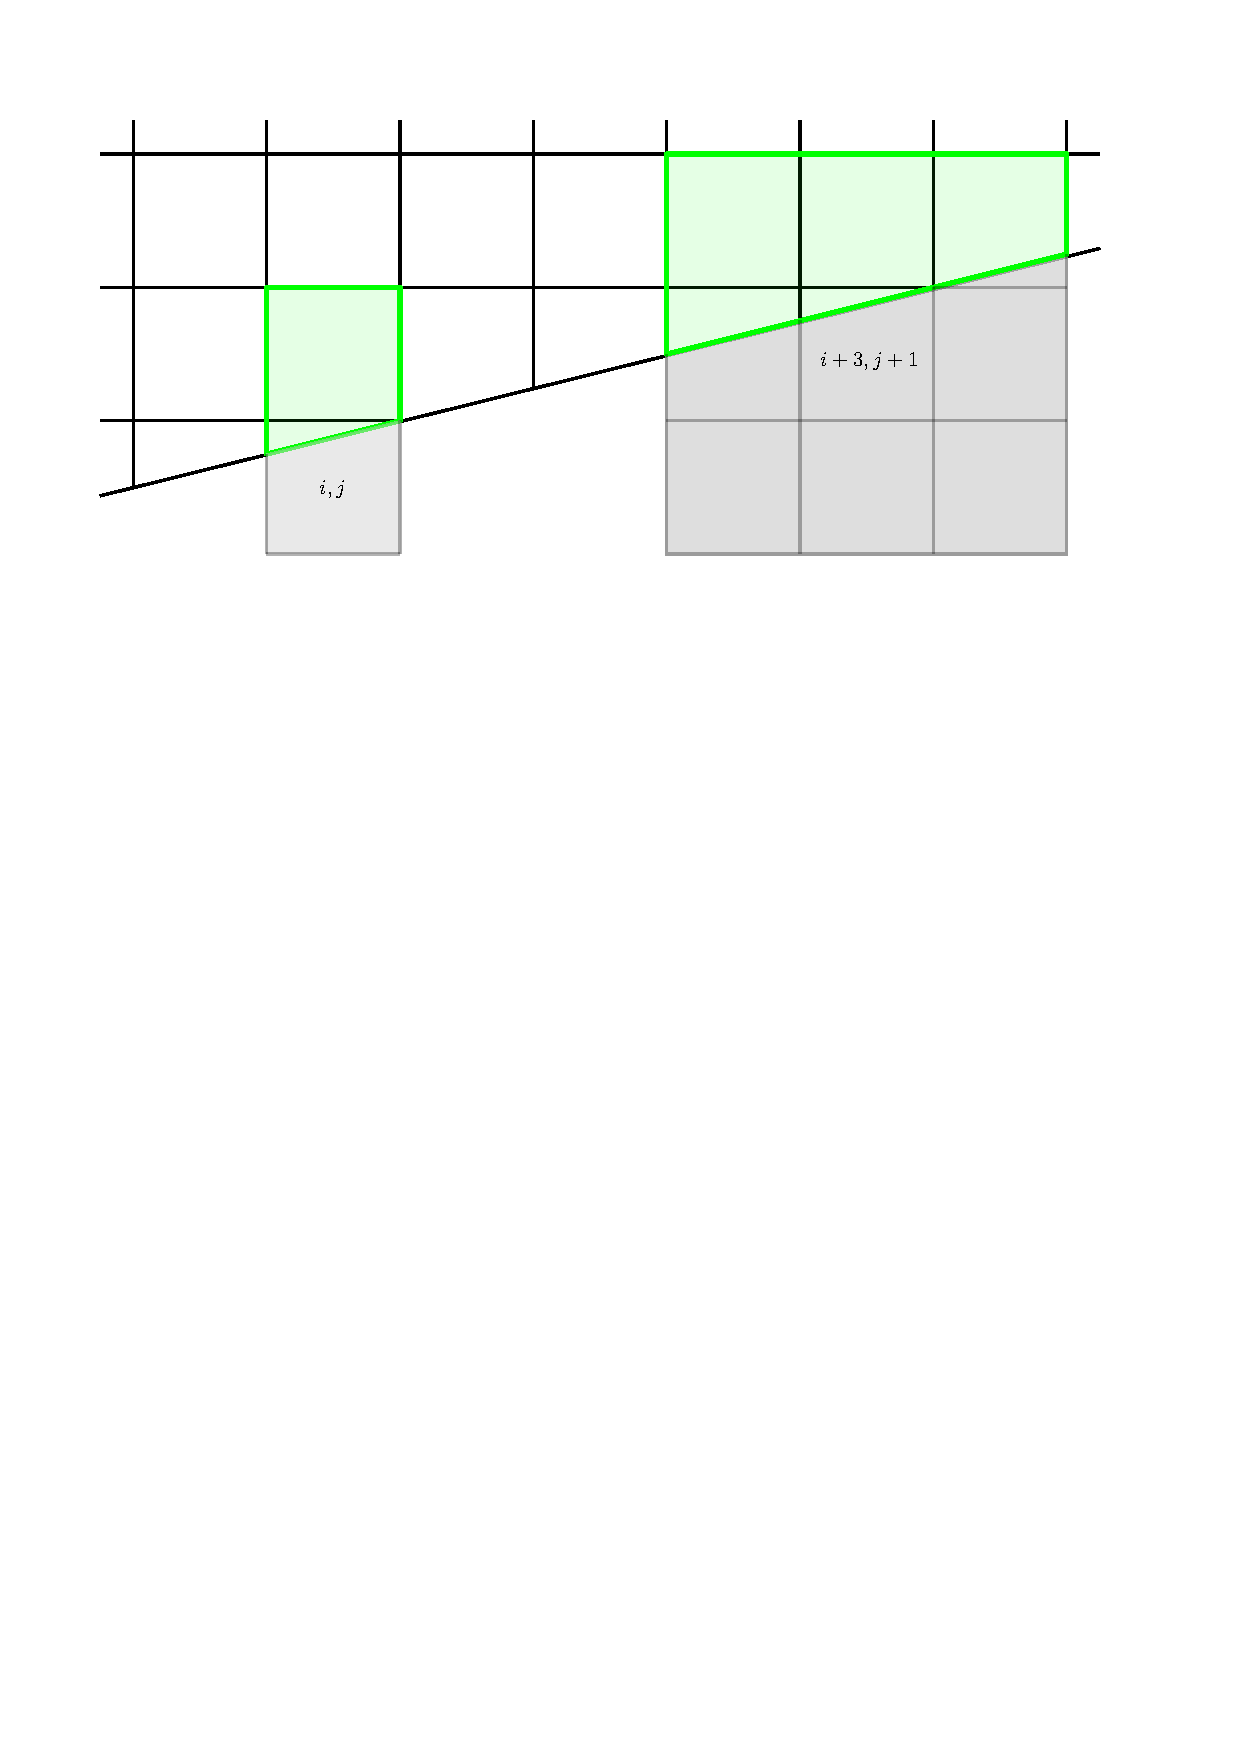
\includegraphics[width=0.5\linewidth]{figs/neighborhoods.pdf}
    \caption{\sf On the left, a small cell is merged with a cell in the direction 
    normal to  the wall.  On the right, a small cell is merged with neighbors that are at most one cell away, i.e., cells located in the $3\times3$ tile.}
    \label{fig:neighborhoods}
\end{figure}

\begin{figure}
	\subfloat[\sf Normal neighborhood (in red) for both small cells in the right corner.]{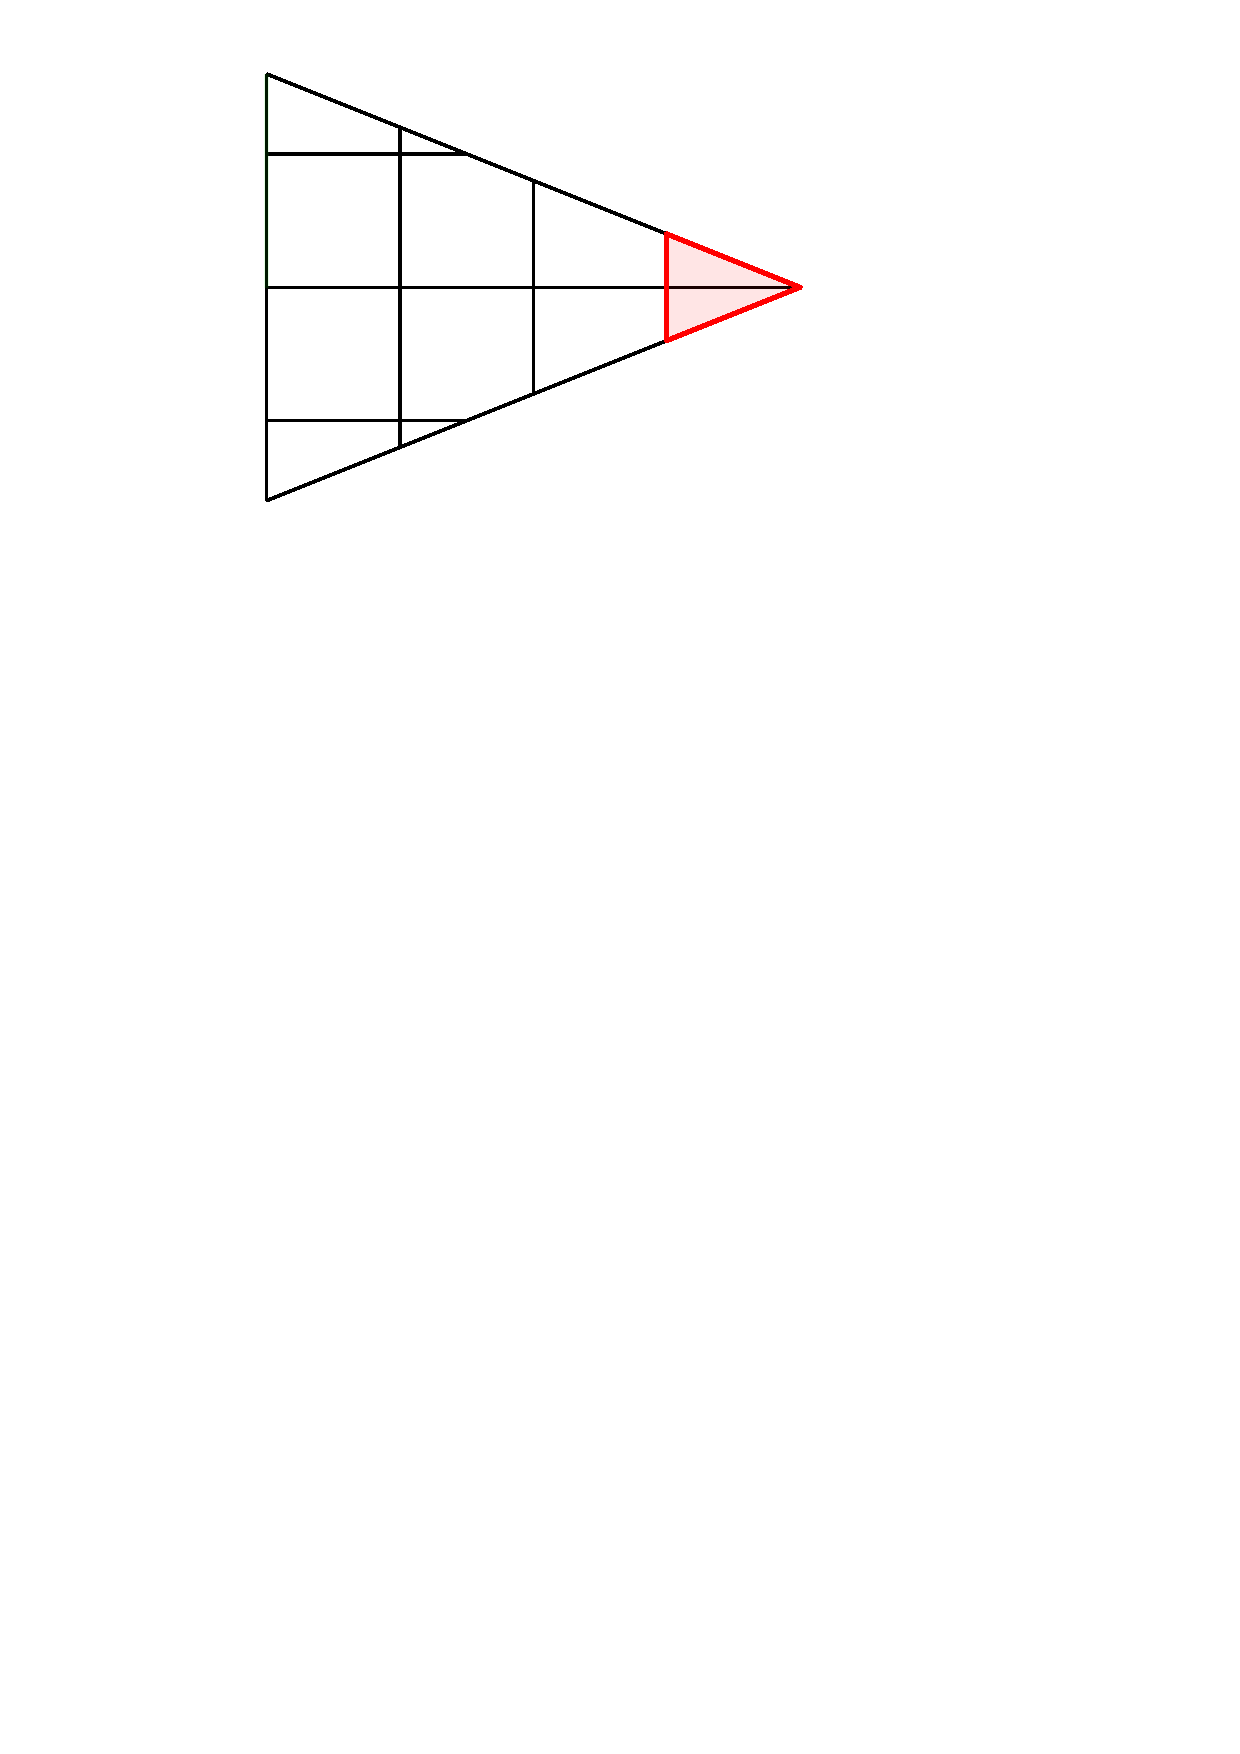
\includegraphics[width=.45\textwidth]{figs/normaldirection1.pdf} \label{fig:normalneighborhood}}
	\hfill
	\subfloat[$3\times 3$ merging neighborhood for both small cells in the right corner.]{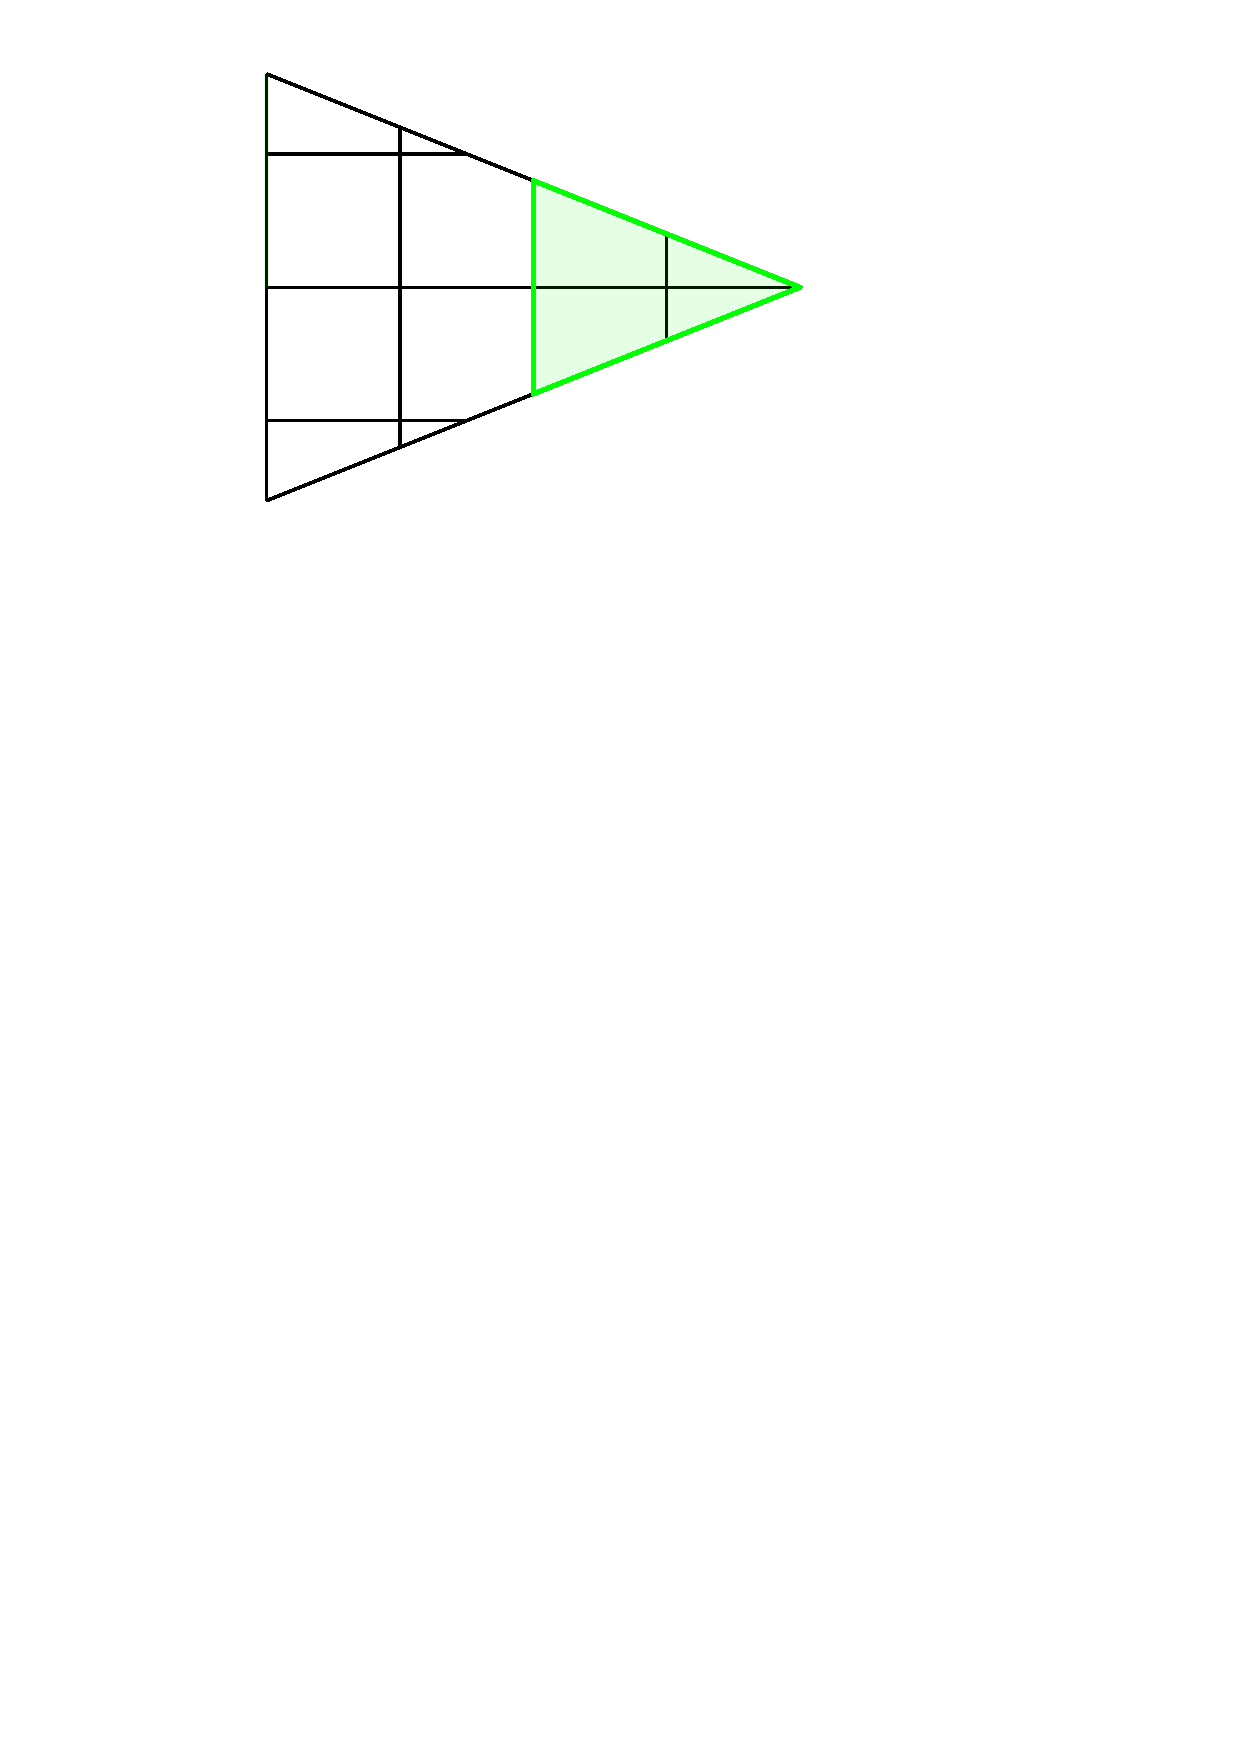
\includegraphics[width=.45\textwidth]{figs/normaldirection2.pdf} \label{fig:3x3neighborhood}}
	\caption{\sf Sometimes, the normal neighborhood is not large enough if a small cell merges with another small cell.  In this case, we use the $3\times 3$ tile, or $5\times5$ neighborhood until the volume constraint \eqref{eq:vmerge} is satisfied.}
\end{figure}
% If the neighboring cell 
% is also cut, it can happen that the
% merged cell is not sufficiently large (SHOW EXAMPLE?). 
% Next we try a 2 by 2
% neighborhood, including the original cut cell. Later we also show
% results using a 3 by 3 neighborhoods. However the larger the
% neighborhood the more diffusive the results.

% Note that this does not have the difficulty of cell merging, since 
% overlapping neighborhoods are allowed. 

\item
{\bf Each cell counts how many neighborhoods it is a part of.}

\vspace*{.1in}
A full cell is its own merging neighborhood, since it has sufficient
volume all by itself. However, we will still refer to all cells as having a
merging neighborhood for ease of presentation.  In figure \ref{fig:overlappingneighs}, we provide an example cut cell mesh with all merging neighborhoods plotted.  We also display the number of overlapping neighborhoods on a cell, this is the neighborhood {\em count} for each cell.
\begin{figure}
	\subfloat[]{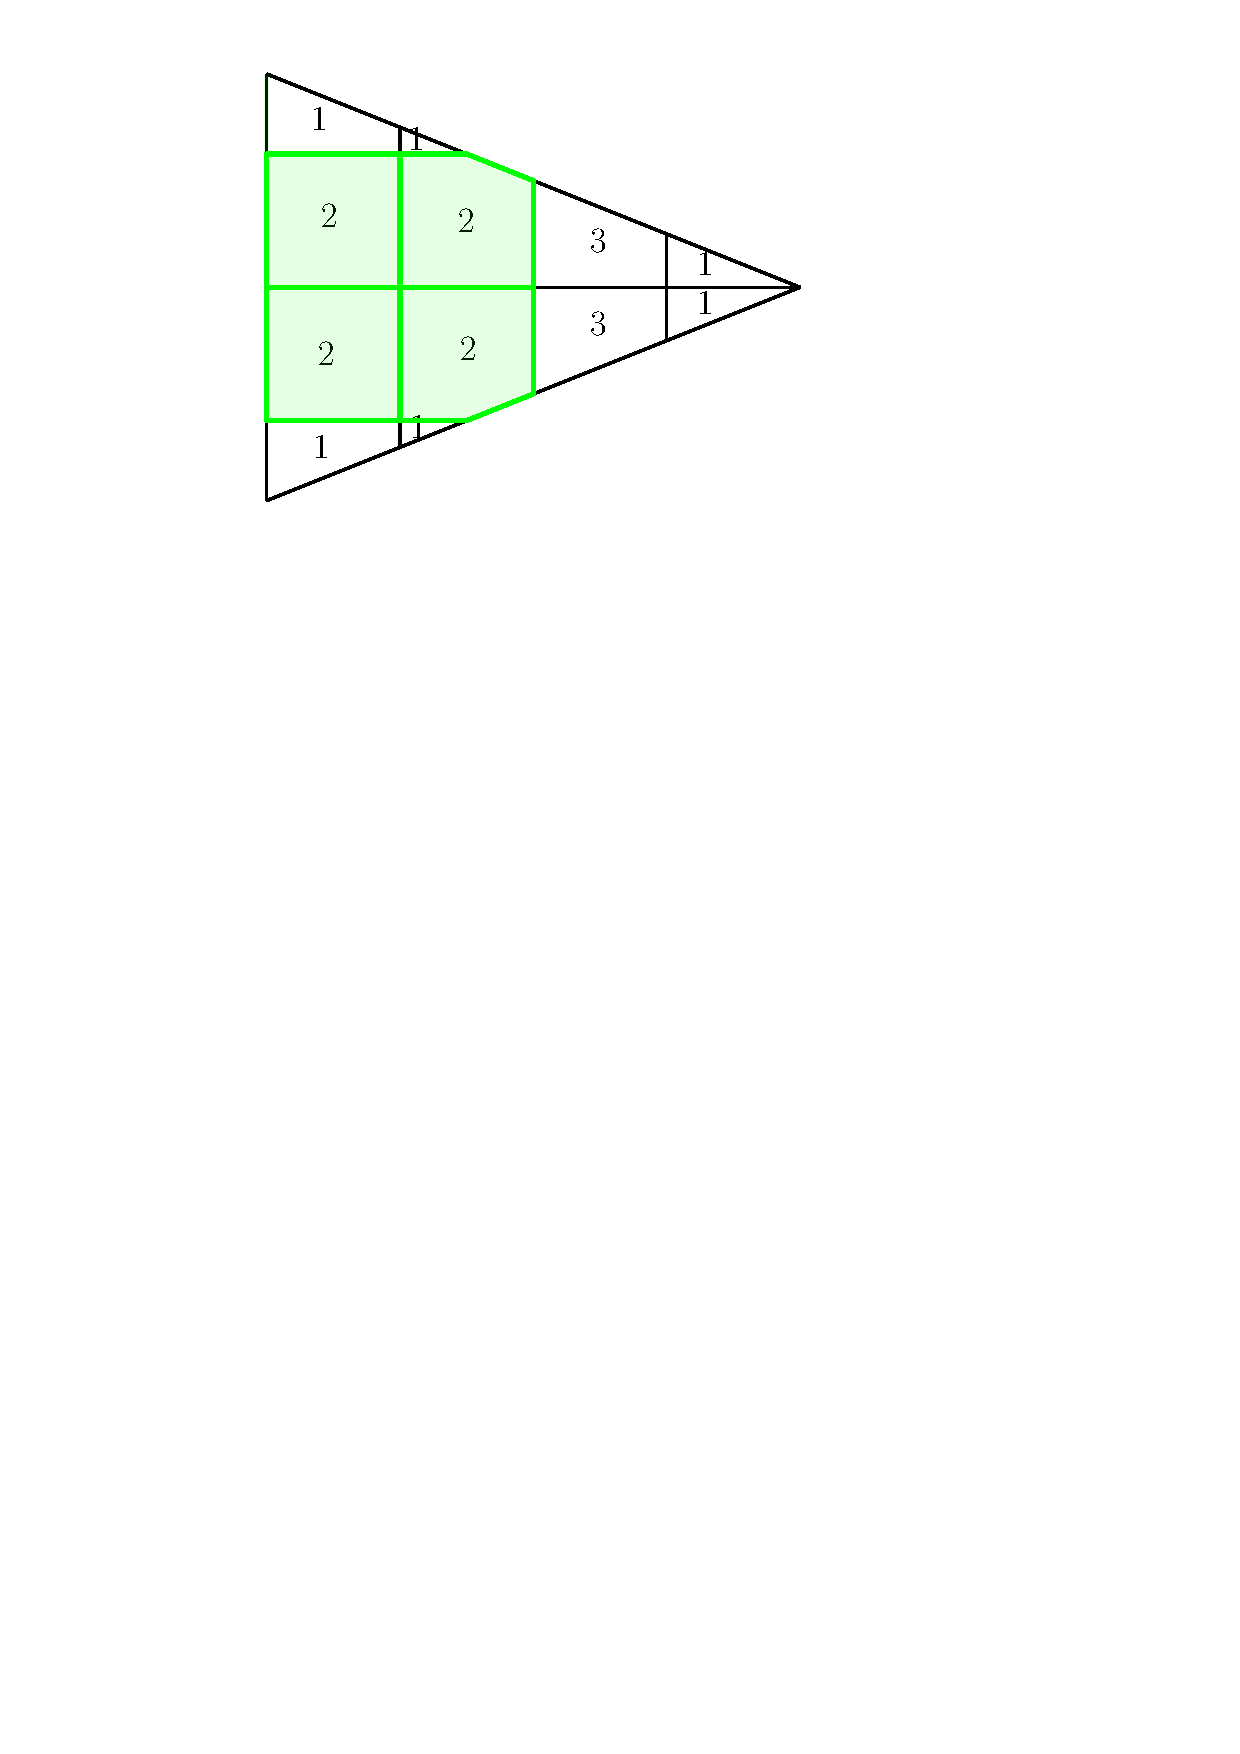
\includegraphics[width=.24\textwidth]{figs/numoverlaps1.pdf} \label{fig:numoverlaps1}}
	\hfill
	\subfloat[]{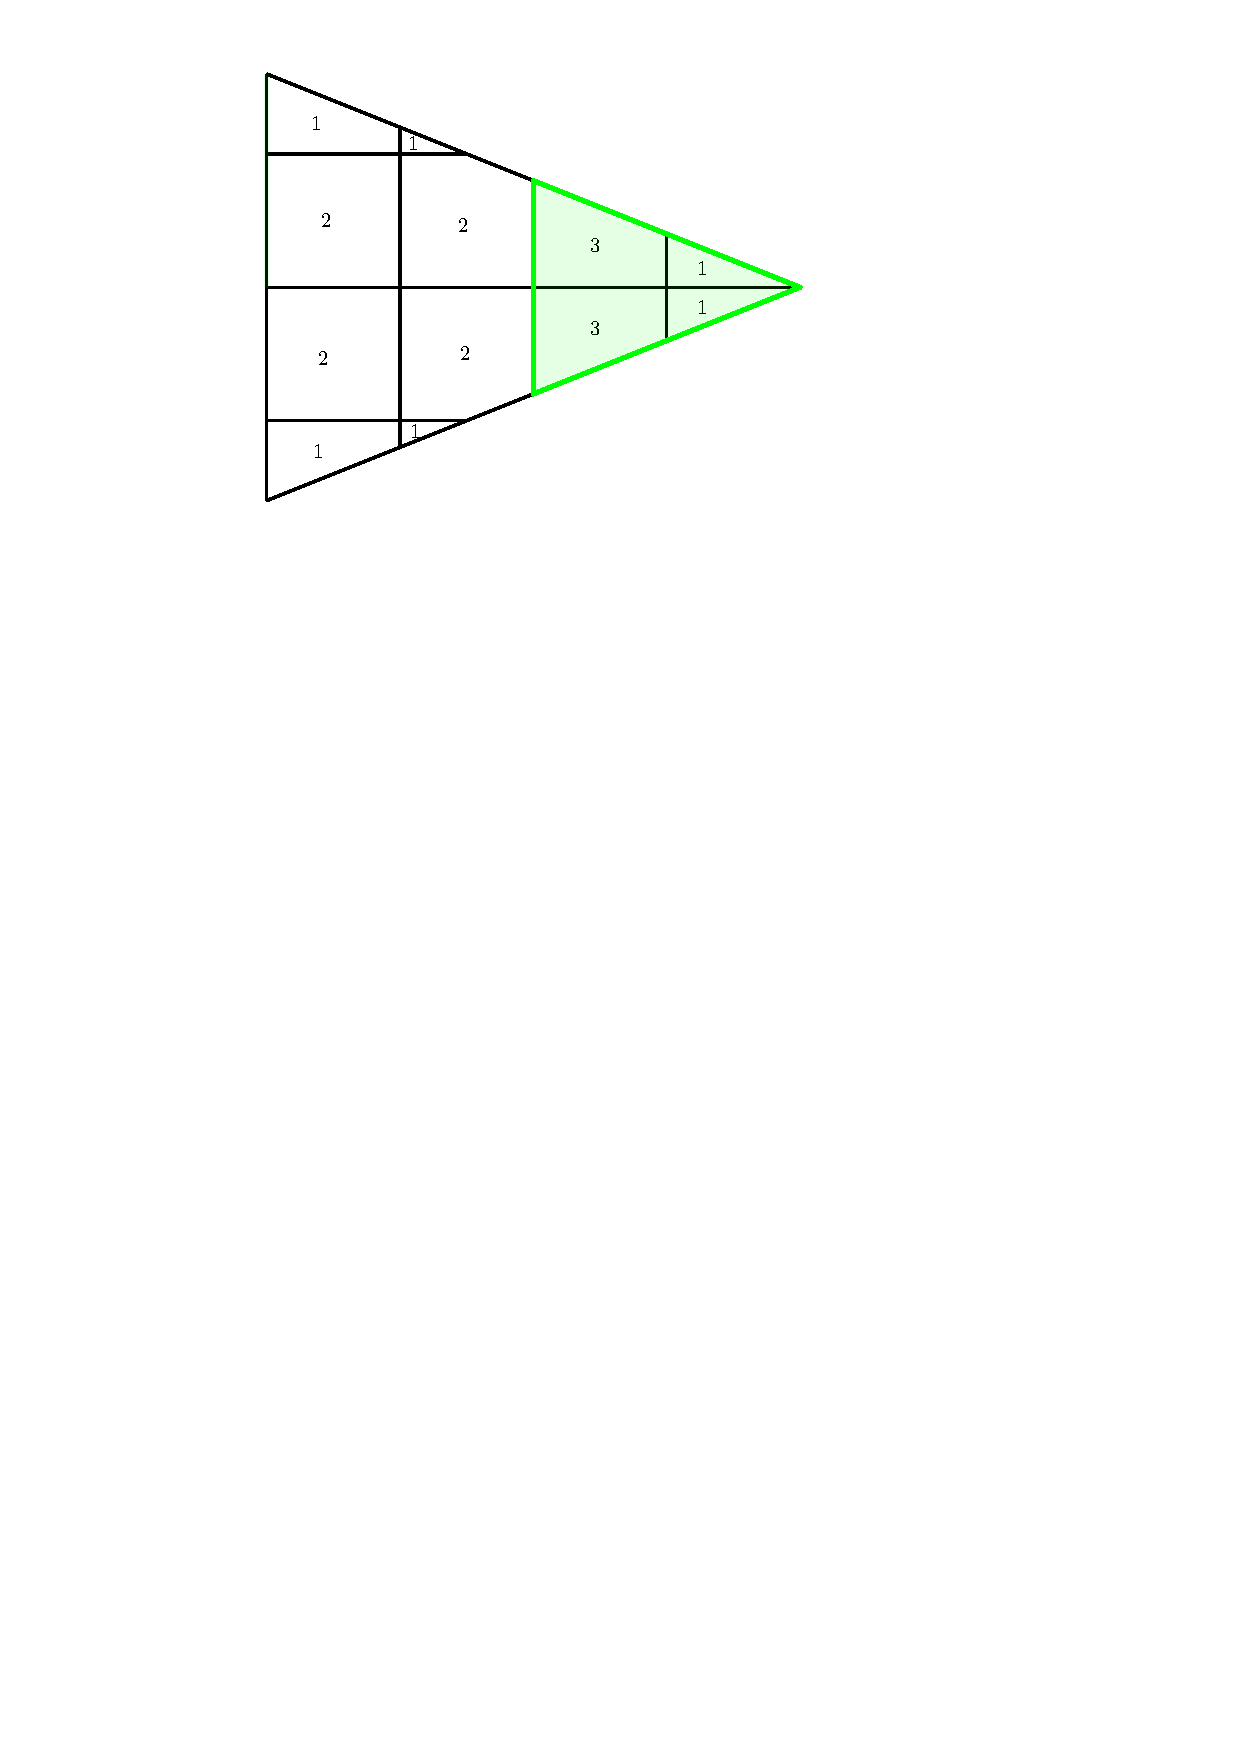
\includegraphics[width=.24\textwidth]{figs/numoverlaps5.pdf} \label{fig:numoverlaps4}}
	\hfill
	\subfloat[]{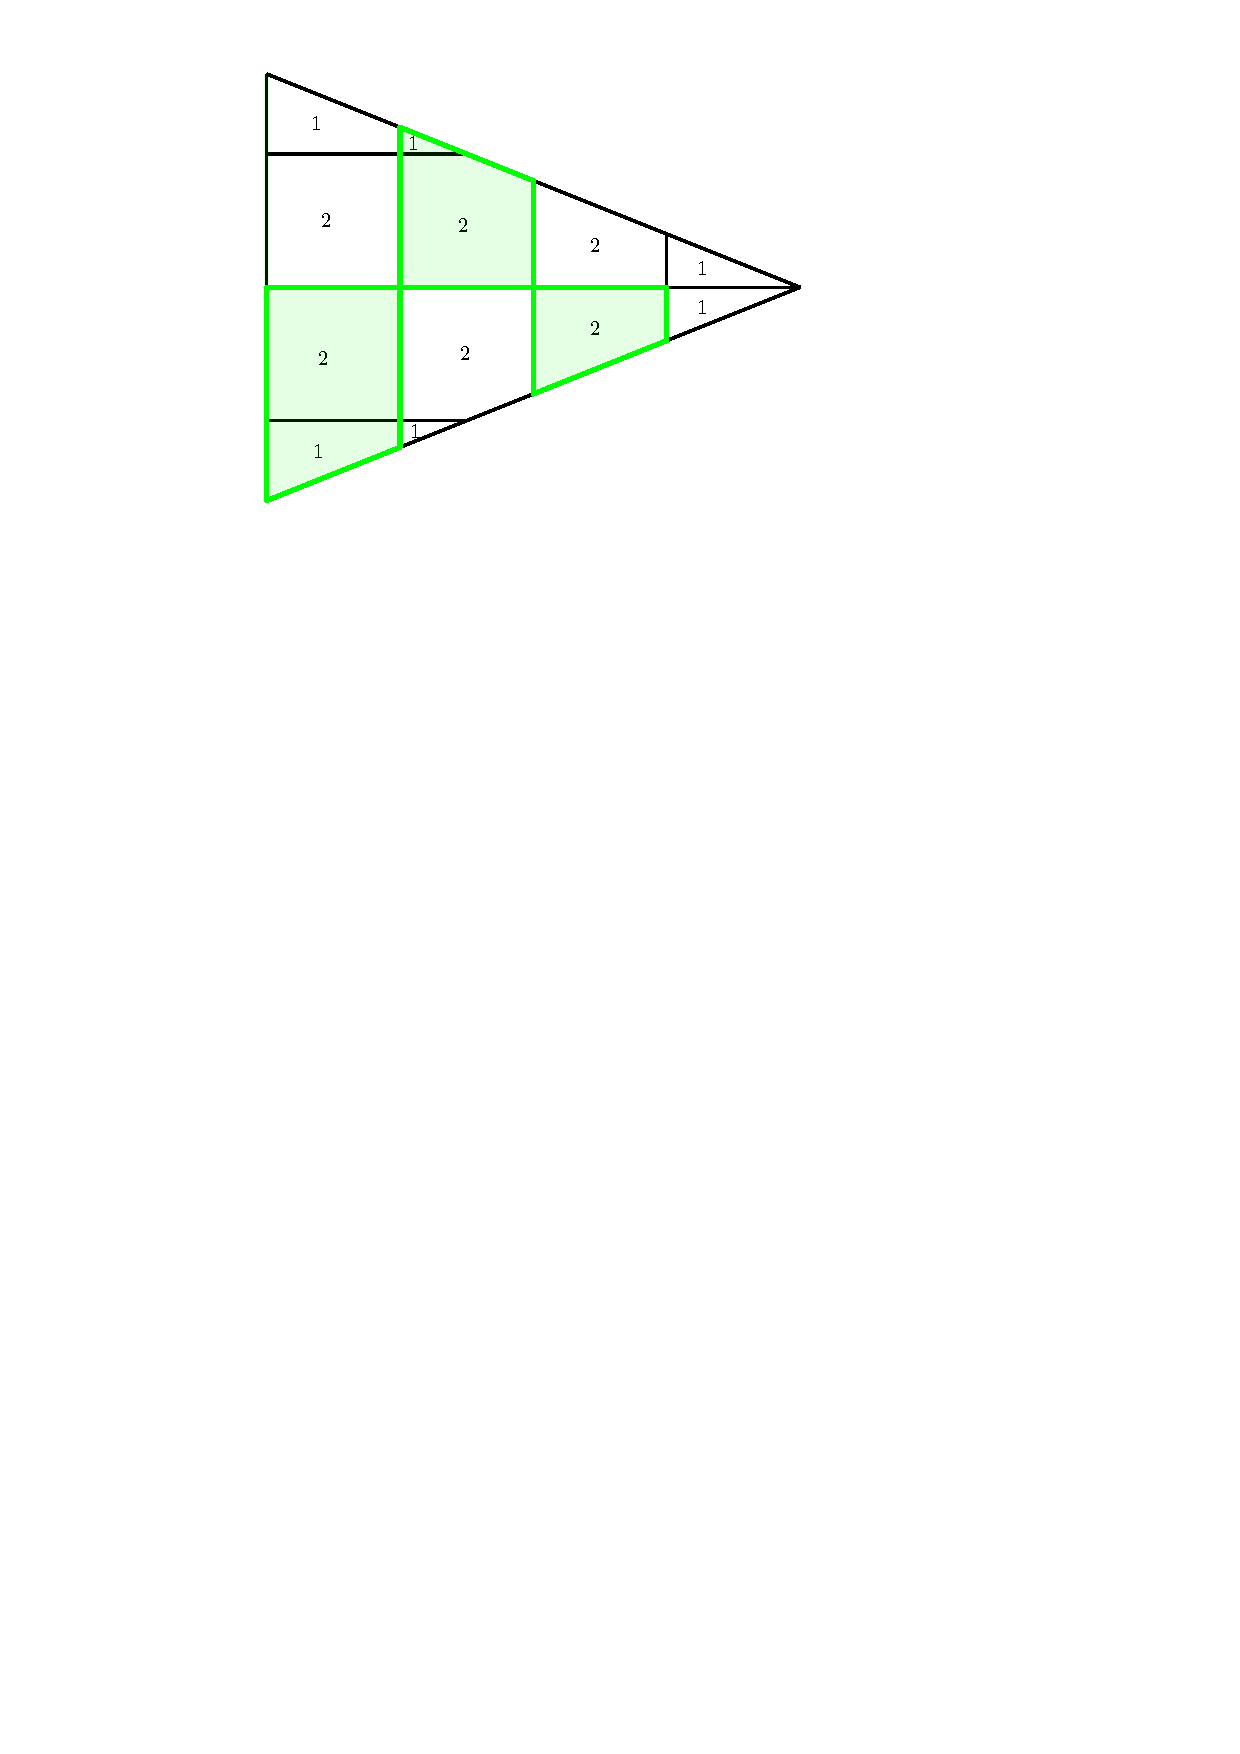
\includegraphics[width=.24\textwidth]{figs/numoverlaps2.pdf} \label{fig:numoverlaps2}}
    \hfill
	\subfloat[]{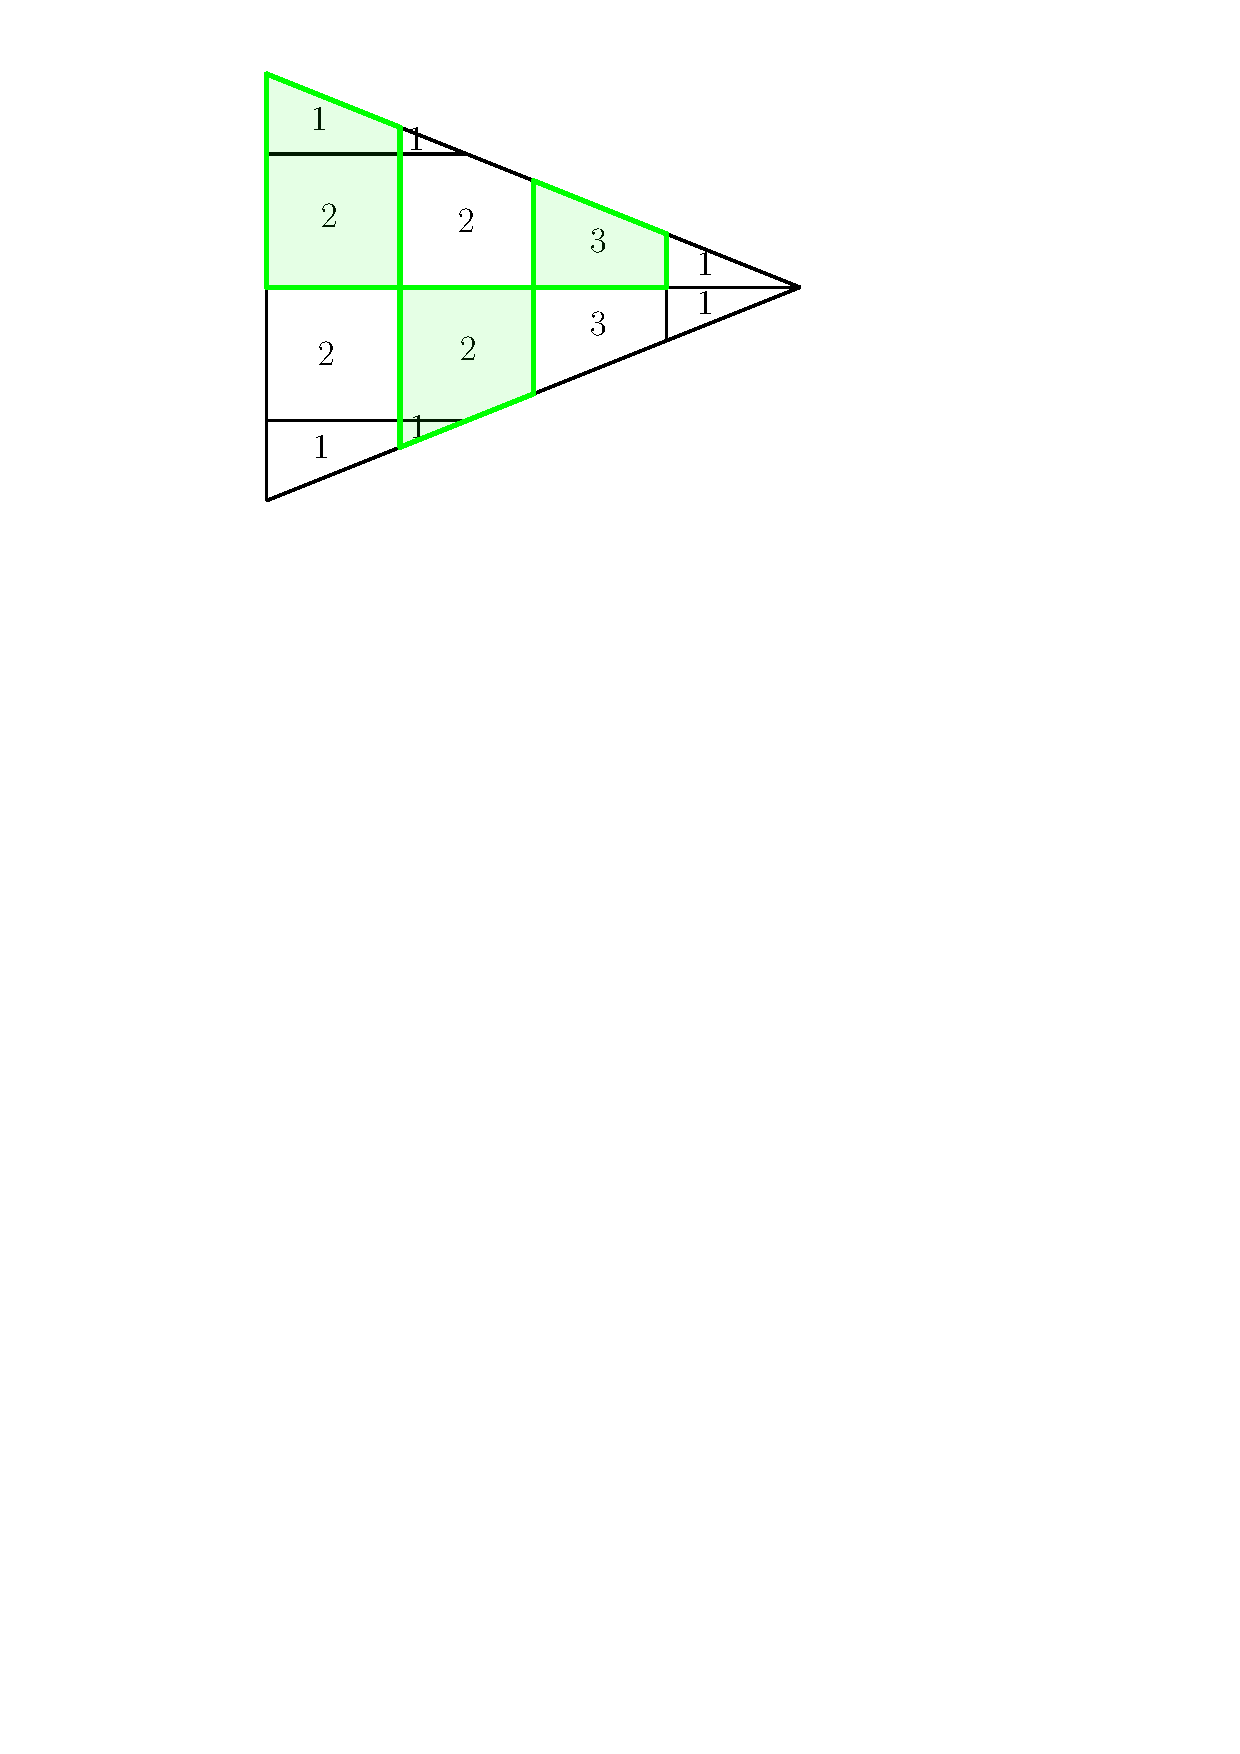
\includegraphics[width=.24\textwidth]{figs/numoverlaps3.pdf} \label{fig:numoverlaps3}}
	\caption{\sf All merging neighborhoods on an example cut cell mesh (in green).  We display the number of overlapping merging neighborhoods on each cell. Note, in figure \ref{fig:numoverlaps4}, there are two merging neighborhoods that occupy the same location, one per small cell in the right corner.} \label{fig:overlappingneighs}
\end{figure}
Note that a full cell
can be part of two or more merging tiles if it is placed next to 
several tiny cut cells. An example is shown in
figure \ref{fig:2nborTile}. The cells in green are part of two
neighborhoods, and those in red are part of three.   
 Most full
cells are only members of their own tile and will have a count of one.
Only cells within a narrow band of the cut cells will have a count
larger than one.


\end{itemize}



% \begin{figure}[h!]
% \begin{center}
% 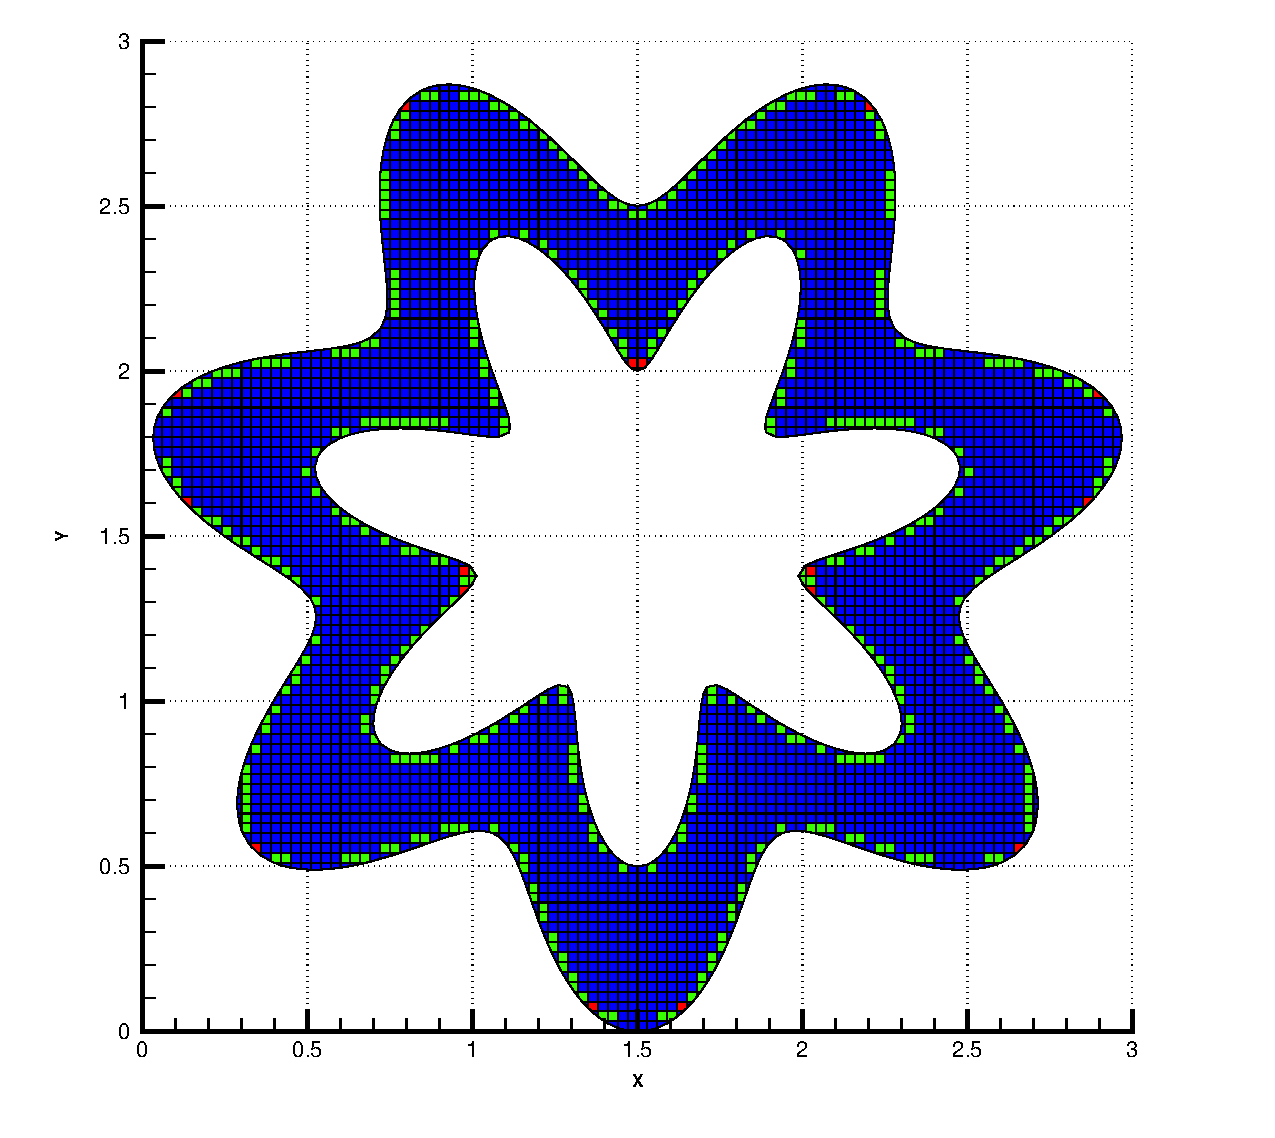
\includegraphics[width=4.5in]{figs/waveynumhoods.eps}
% \caption{\sf Domain from example XX.  Figure shows how many
% neighborhoods each cell belongs to: 
% one (white), two (blue), or three (red).
% The full example is shown in section \ref{sec:compResults}.}
% \label{fig:2nborTile}
% \end{center}
% \end{figure}

The two steps above can be part of a preprocessing step, since they do not
depend on the computed solution. For moving geometry however they would
be done at each step.
Using the merging tiles and the cell counts, the state redistribution
algorithm after one time step or stage is as follows:

%\begin{enumerate}[label=Step \arabic*:,leftmargin=2\parindent]
\begin{enumerate}
\item
{\bf Compute the volume-weighted and count-weighted solution for all
merged tiles.}   

\vspace*{.1in}
The contribution of each cell is divided by the number of neighborhoods 
it is part of (i.e. its count). The notation in this section refers
to cut cell $i,j$, with solution $U_{i,j}$ and volume
$V_{i,j}$. 
The provisionally updated solution before the
stabilization algorithm is applied is $\widehat{U}_{i,j}$.
There will now be many temporary merging neighborhoods which 
we denote as $\widehat{Q}_{i,j}$. 
Let $M_{i,j}$ denote the set of cell indices in the cell $(i,j)$ merging
neighborhood.  Then
\begin{equation}
\label{tiledef}
\widehat{Q}_{i,j} =  \frac{1}{{\widehat V}_{i,j}} \, \sum_{k \in M_i} \,  
\frac{V_k}{N_k}  \,\,  \widehat{U}_k
\end{equation}
where the volume ${\widehat V}_{i,j}$ is the merging tile volume similarly weighted,
\begin{equation}
\label{voldef}
{\widehat V}_{i,j} =  \sum_{k \in M_i } \,  \frac{V_k}{N_k}  .
\end{equation}

In other words, the contributions from each cell are weighted by the
number of neighborhoods they contribute to.
In the above equations, $k$ is  a multi-index ranging over the neighbors 
of cell $i,j$ included in its merging tile.
Note that most full cells will have ${\widehat V}_{i,j} = V_{i,j}$, 
and $\widehat{Q}_{i,j}  = \widehat{U}_{i,j}$.





\item
{\bf Compute a (limited) gradient for each merging
tile.}

\vspace*{.1in}
For cut cells, a least squares procedure  similar to the one used for
the finite volume update is an obvious choice. However instead of using the
solution $U_{i,j}$ on the Cartesian mesh at time $t_n$,
the merging neighborhood solution  $\widehat{Q}_{i,j}$ is used. It is important
to note that the centroid of the merging neighborhood is \textit{not} the centroid of cell ${i,j}$ (figure \ref{fig:centroids}).
\begin{figure}
    \centering
    \subfloat[]{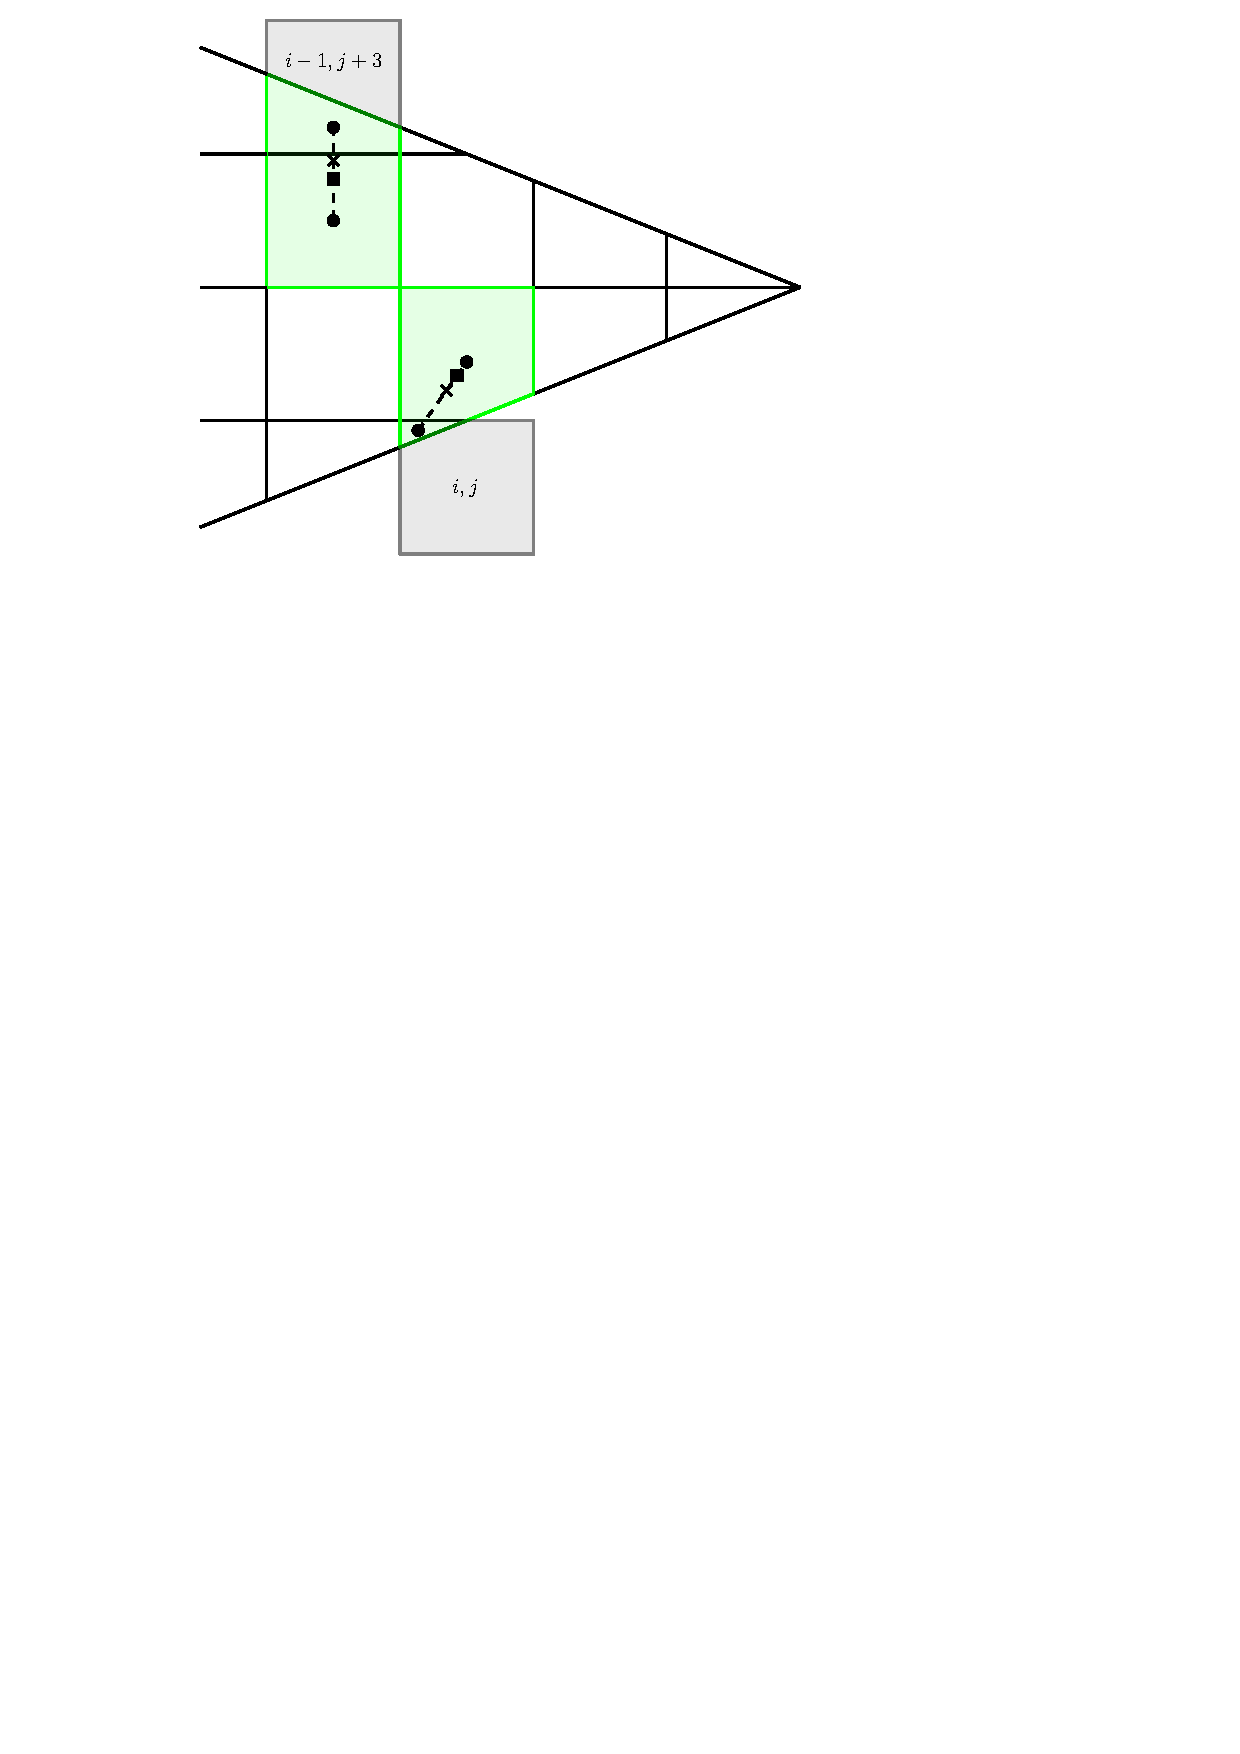
\includegraphics[width=0.45\linewidth]{figs/centroids3.pdf}} \hfill
    \subfloat[]{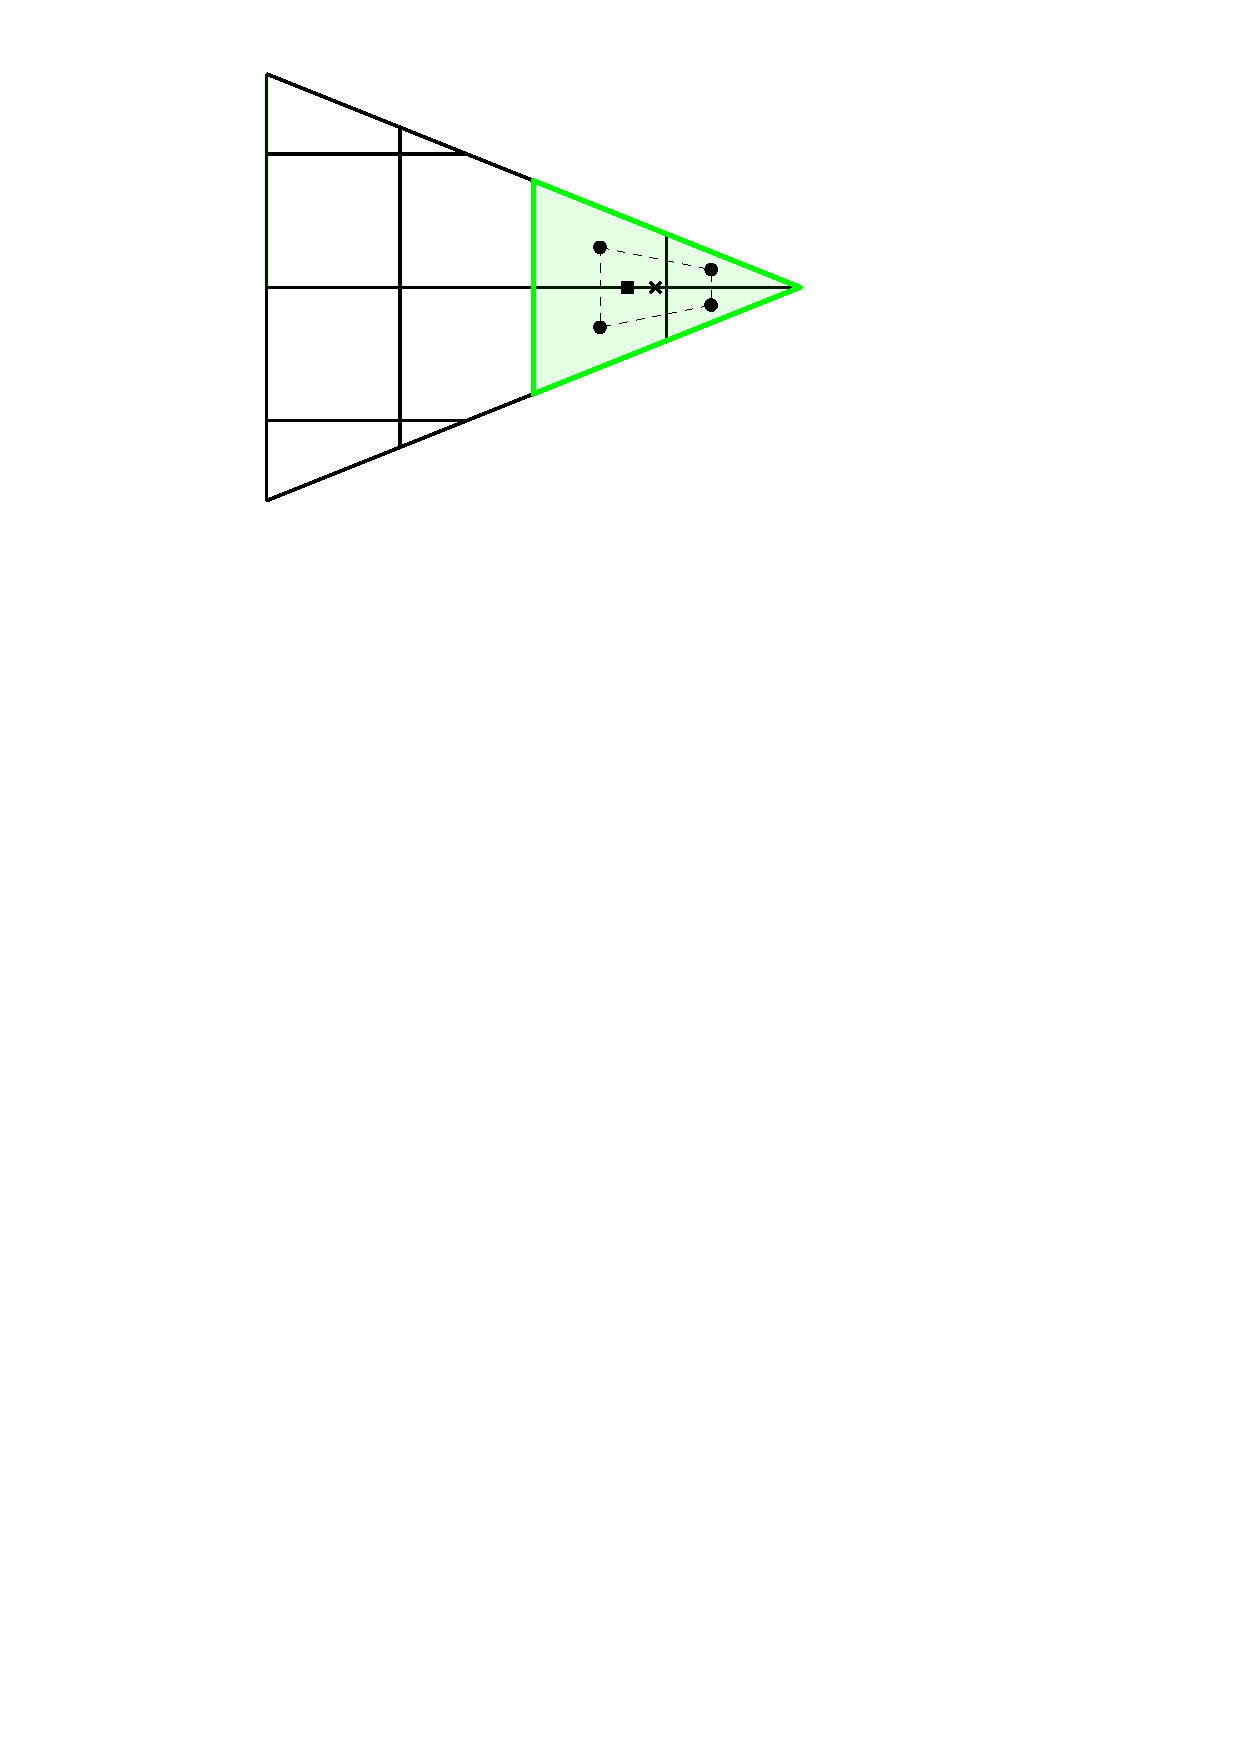
\includegraphics[width=0.45\linewidth]{figs/centroids4.pdf}}
    \caption{\sf The centroids of the Cartesian and cut cells are indicated with a solid circle ($\bullet$).  The centroids and weighted centroids of the merging neighborhoods are indicated with a square ($\blacksquare$) and a cross ($\times$), respectively. Note that the centroids and weighted centroid of the cut cell neighborhoods do not necessarily coincide.}
    \label{fig:centroids}
\end{figure}
The reconstruction neighborhood for $i,j$ is initialized to the $3 \times 3$ tile centered on $i,j$.
With this choice, it could happen that the centroids are too close to each other to compute a gradient in the normal direction (figure \ref{fig:tooclose}). If the weighted centroids are not at least $0.5\,\Delta x$  and $0.5\,\Delta y$ apart in the $x$ or $y$ direction then we increase the stencil size for the gradient computation.  For example, if the weighted centroids are too close in the $x$ direction, but not the $y$ direction, then the $5\times 3$ tile is used as the reconstruction neighborhood.  Similarly, if the weighted centroids are too close in the $y$ direction, but not the $x$ direction, then the $3\times 5$ tile is used as the reconstruction neighborhood.  The neighborhood size is increased until the distance constraint is satisfied in both directions.  In figure \ref{fig:tooclose}, the appropriate reconstruction neighborhood is $3\times 5$ reconstruction tile.
% The same neighborhood that is used for computing the gradient can be used to limit the gradient to prevent overshoots. The centroid is computed using the same weighting by number of neighborhoods as when the volume was computed. (IS THIS TRUE AND IS IT NECESSARY) NEED DISCUSSION OF NOT A REAL CENTROID
% For most full cells with a count of one, the normal gradient computation as done in the finite volume update will suffice.

\begin{figure}
    \centering
    \subfloat[]{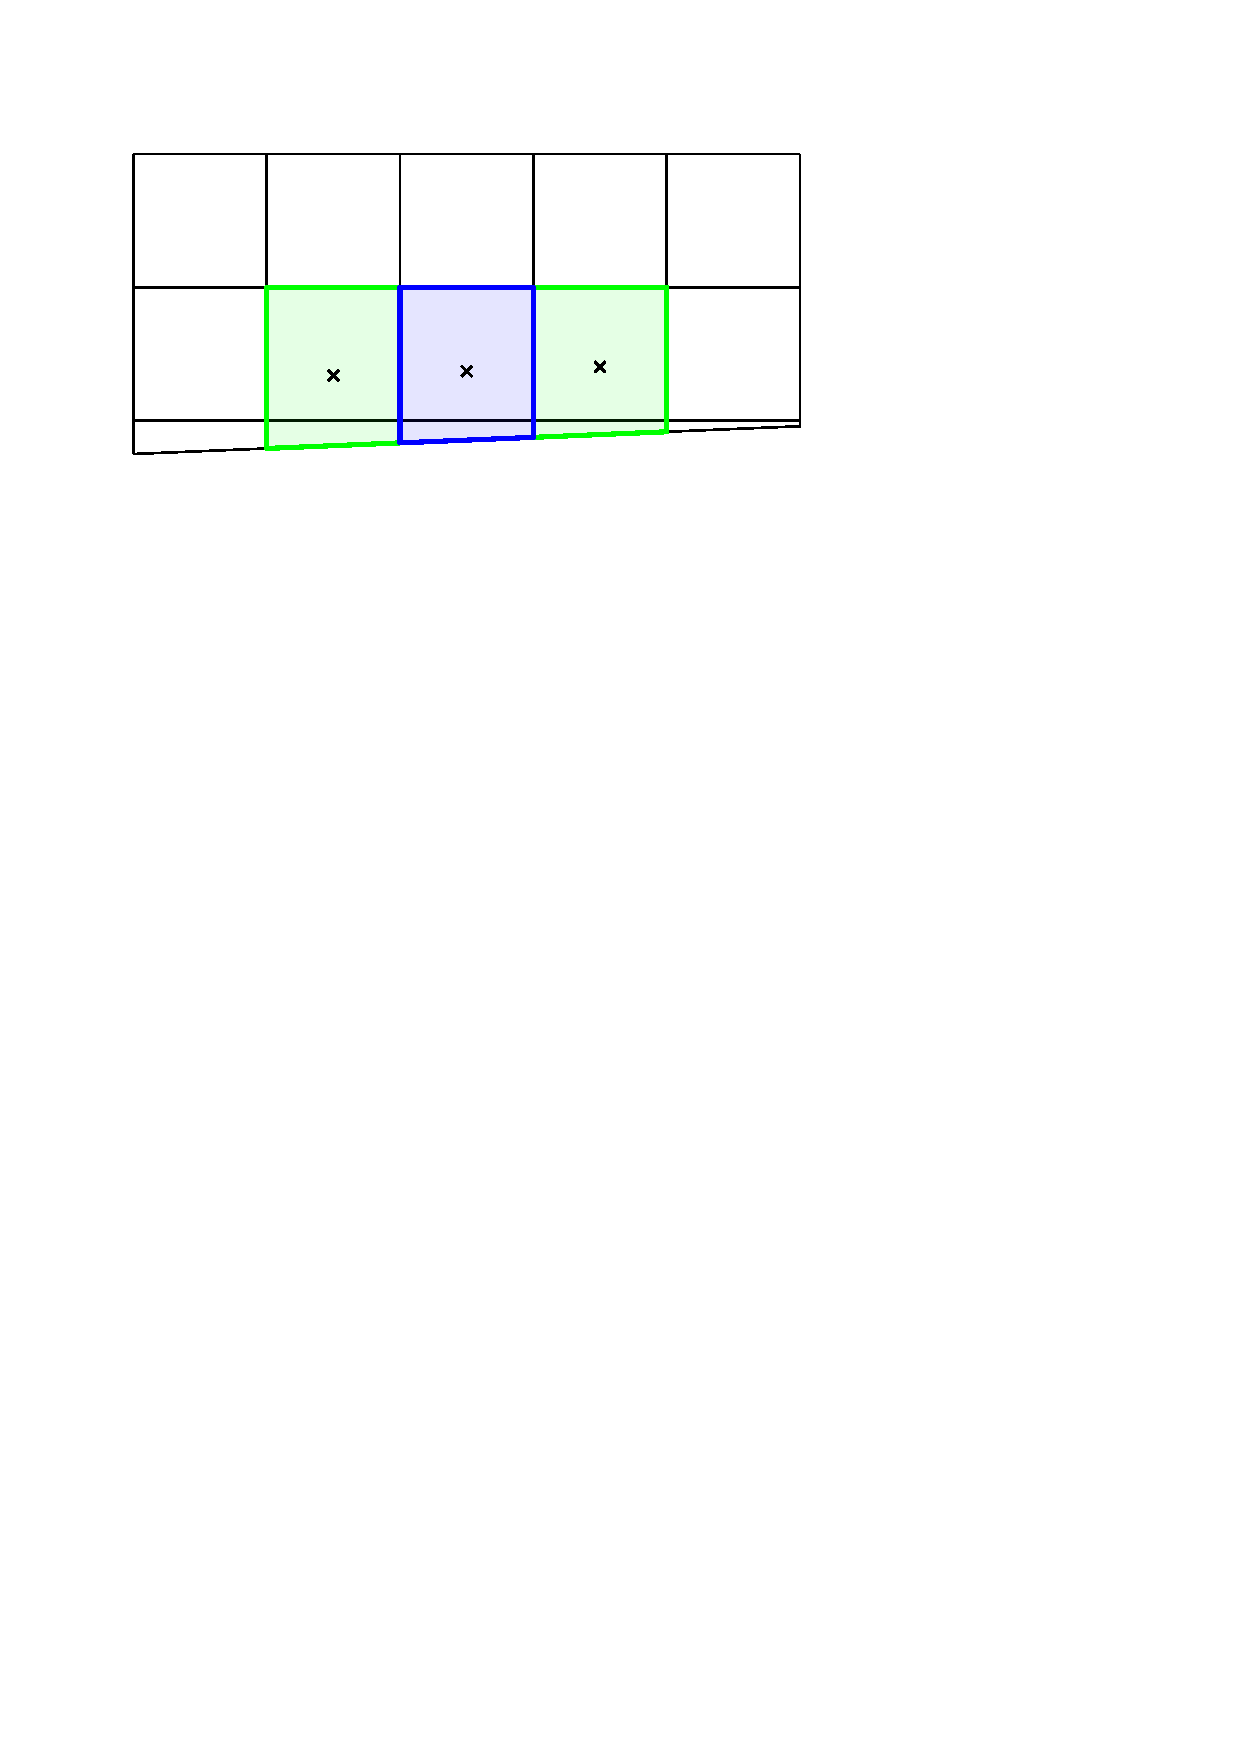
\includegraphics[width=0.45\linewidth]{figs/tooclose2.pdf}} \hfill
    \subfloat[]{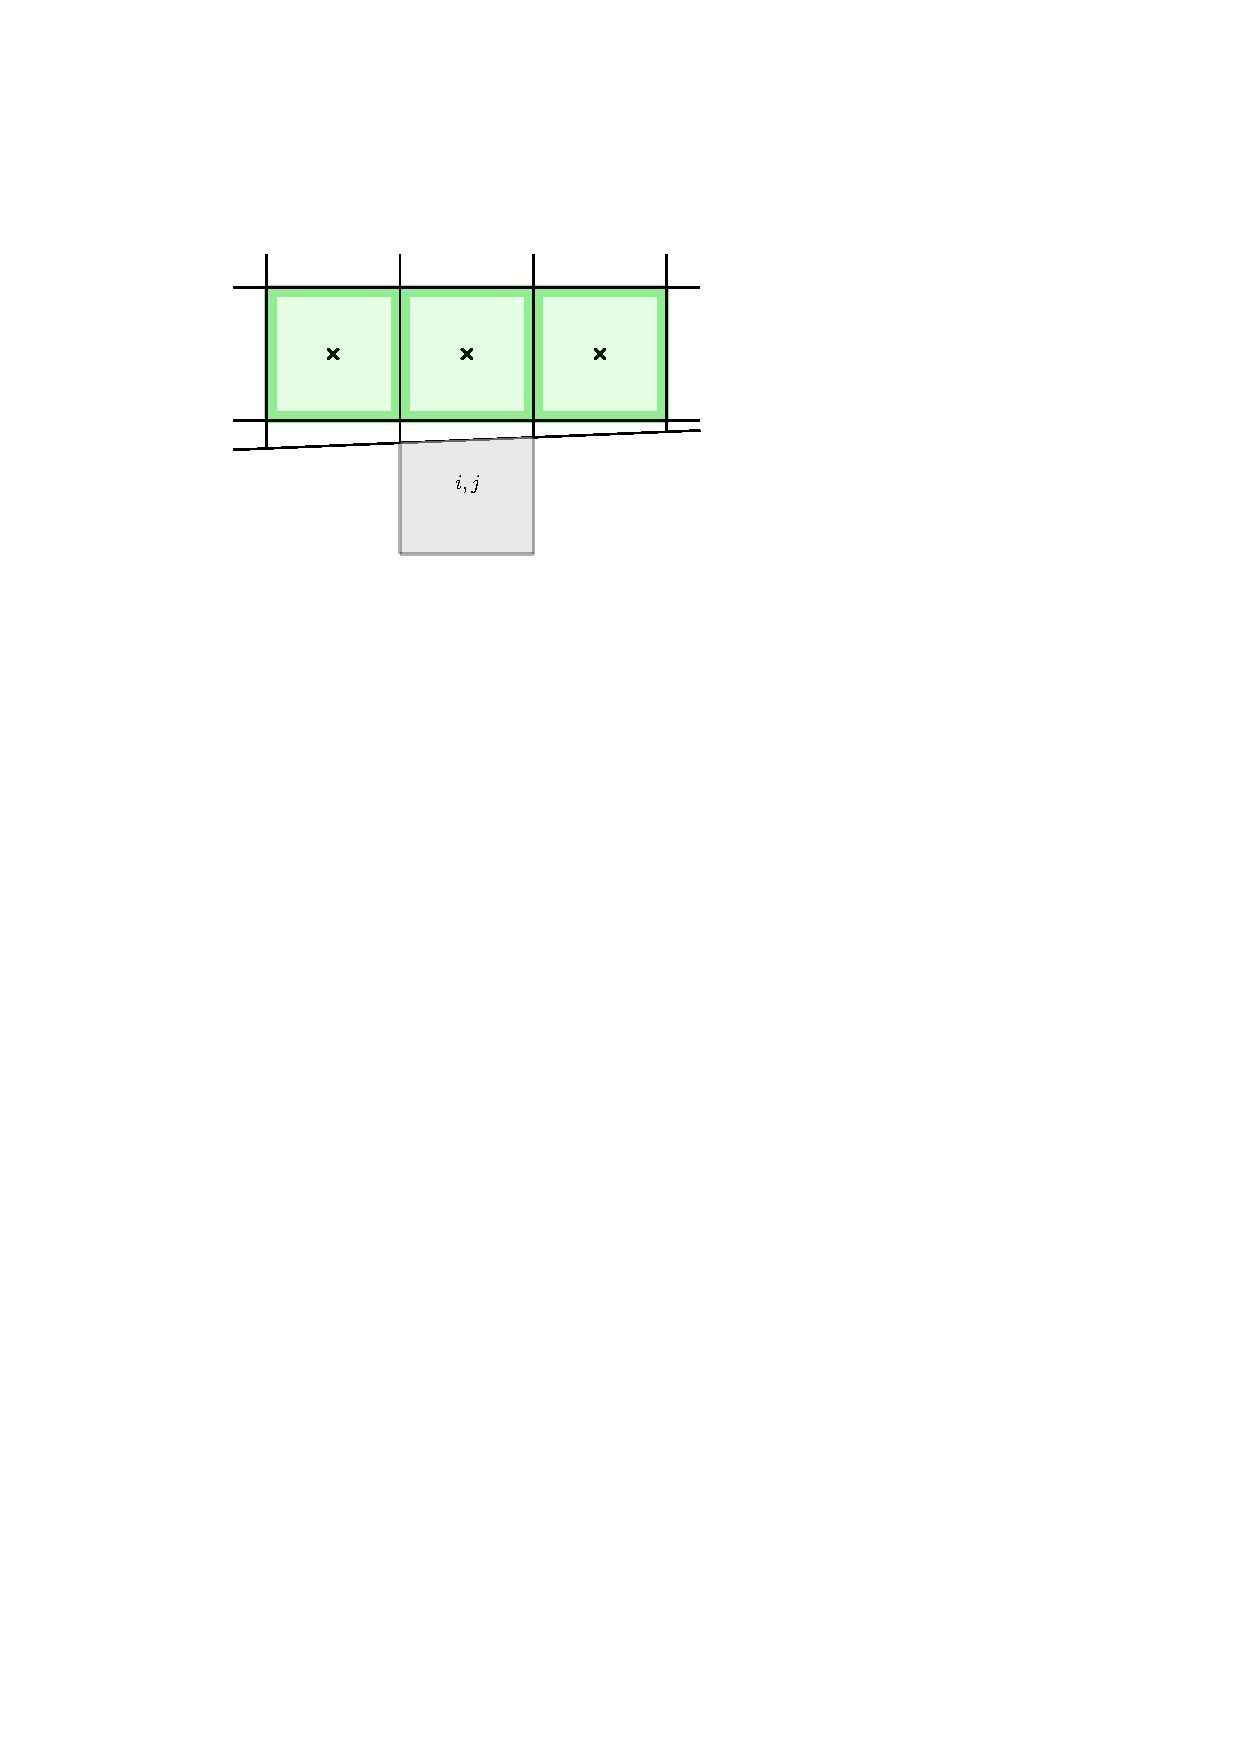
\includegraphics[width=0.45\linewidth]{figs/tooclose1.pdf}} 
    \caption{\sf The blue cell's $3\times3$ reconstruction tile highlighted in green.  The weighted centroids are indicated with a cross ($\times$).}
    \label{fig:tooclose}
\end{figure}

\item
{\bf Replace the provisionally computed cut cell values and their adjacent
full cell neighbors with  the contributions from the merged tiles.} 

\vspace*{.1in}
The final solution at time $t^{n+1}$ on cut cell $i,j$ is obtained by compiling a the indices of all merging neighborhoods that overlap cell $i,j$ in the set $W_{i,j}$.  Then, the solution on merging neighborhood $k,l$ in $W_{i,j}$ is evaluated at $i,j$'s physical centroid, $x_{i,j}$, given by $\hat{q}_{k,l}(x_{i,j})$.  The final solution value on cell $i,j$ is given by the average of these values, i.e.,
\begin{equation} \label{eq:final_update_linear}
U^{n+1}_{i,j} := \frac{1}{N_{i,j}}\sum_{(k,l) \in W_{i,j}}\hat{q}_{k,l}(x_{i,j}).
\end{equation}
To use the example of figure \ref{fig:2nborTile}, the cut cell value
\begin{equation}
   U_{i,j}^{n+1} := \widehat{Q}_{i,j} 
   + (x_m - x_{i,j}) \, \frac{\partial \widehat{Q}_{i,j}}{\partial x} 
   + (y_m - y_{i,j}) \, \frac{\partial \widehat{Q}_{i,j}}{\partial y}
\end{equation}
since cell ${i,j}$ only belongs to one neighborhood. The adjacent full cell
on the other hand belongs to two neighborhoods -- the one it shares with
the cut cell $i,j$ , and its own merging neighborhood.
So its solution at time $t_{n+1}$  becomes
\begin{equation}
\label{eqn:numhood2ex}
\begin{split}
   U_{i,j+1}^{n+1} \,=\, & \frac{1}{2}\widehat{q}_{i,j}(x_{i,j})+ \frac{1}{2} \widehat{q}_{i,j+1}(x_{i,j}), \\
   = &\frac{1}{2} \left
   (\widehat{Q}_{i,j} 
   + (x_m - x_{i,j+1}) \, \frac{\partial \widehat{Q}_{i,j}}{\partial x} 
   + (y_m - y_{i,j+1}) \, \frac{\partial \widehat{Q}_{i,j}}{\partial y} \right ) + \frac{1}{2} \widehat{Q}_{i,j+1} .
\end{split}
\end{equation}
The last term  in eq. \eqref{eqn:numhood2ex} has no gradient terms because the
centroids of the original cell and merged cell are identical.
The fraction $\frac{1}{2}$ is because cell $(i,j+1)$ is part of  two
neighborhoods, so each contributes half of the solution.
\end{enumerate}

Different choices of neighborhoods, the minimum volume for the merging
neighborhood, gradient neighborhoods, and limiting will give
somewhat different computational results. Some of these will be examined
theoretically using model problems in one space dimension in section
\ref{sec:theory}. These choices can affect the stability limit of the
overall method.
We will also show computational results using different neighborhood
choices in section \ref{sec:compResults} in two space dimensions.

The conservation properties of the algorithm will be discussed after the
higher order SRD algorithm is presented in the next
section (PR PUT IT HERE). It will also be prseented more generally.   
OTHER THINGS HERE? DEMONSTRATE LINEARLY EXACT SECOND ORDER CONVERGENCE
HERE INSTEAD OF COMPRESULTS SECTION?

% SOMEHWERE PUT IMPLEMENTATION SUBSECTION OR AT LEAST A PARAGRAPH
% TO NOTE THAT THE CELL DOESNT KNOW WHO GIVES TO
% IT, SO THIS LOOP IS OVER GIVERS  NOT RECEIVERS.
The final update formula \eqref{eq:final_update_linear} can easily be implemented with a nested for loop in algorithm \ref{alg:finalupdate}.  
The outer loop iterates over the merging neighborhoods $i,j$ and the inner loop iterates over each cell $k,l$ in merging neighborhood $i,j$.  Each merging neighborhood $i,j$ gives a contribution $ \hat{q}_{i,j}(x_{k,l})/N_{k,l} $ to the cells $k,l$ that belong to it.
\begin{algorithm}[H]
\SetAlgoLined
$U^{n+1}(:,:) := 0$\\
 \ForAll{$i,j$}{
     \ForAll{$(k,l) \in M_{i,j}$}{
        $U^{n+1}(k,l) := U^{n+1}(k,l) + \hat{q}_{i,j}(x_{k,l})/N_{k,l} $
     }
 }
 \caption{\sf Final solution update} \label{alg:finalupdate}
\end{algorithm}

\begin{figure}
	\subfloat[]{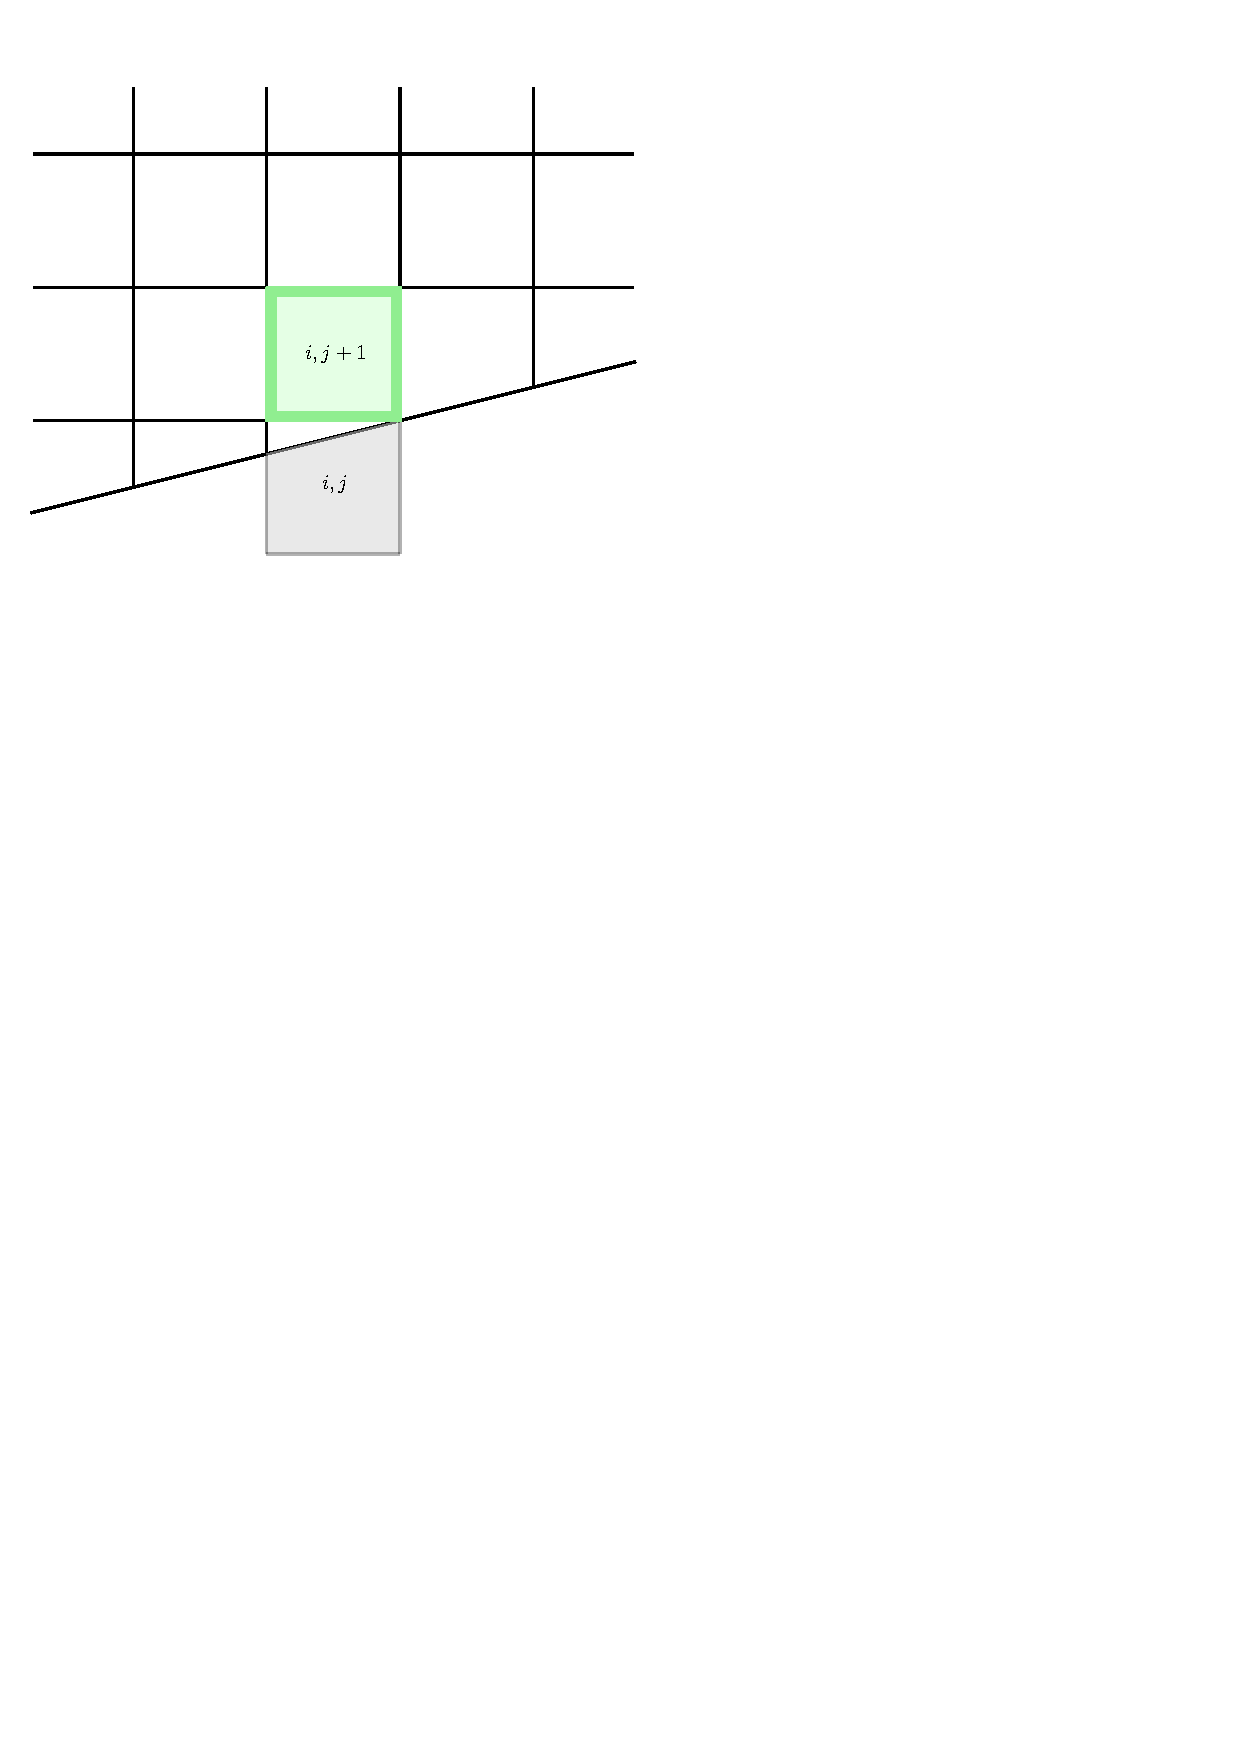
\includegraphics[width=0.45\textwidth]{figs/modelexample2D_1.pdf} \label{fig:2nborTile1}}
	\hfill
	\subfloat[]{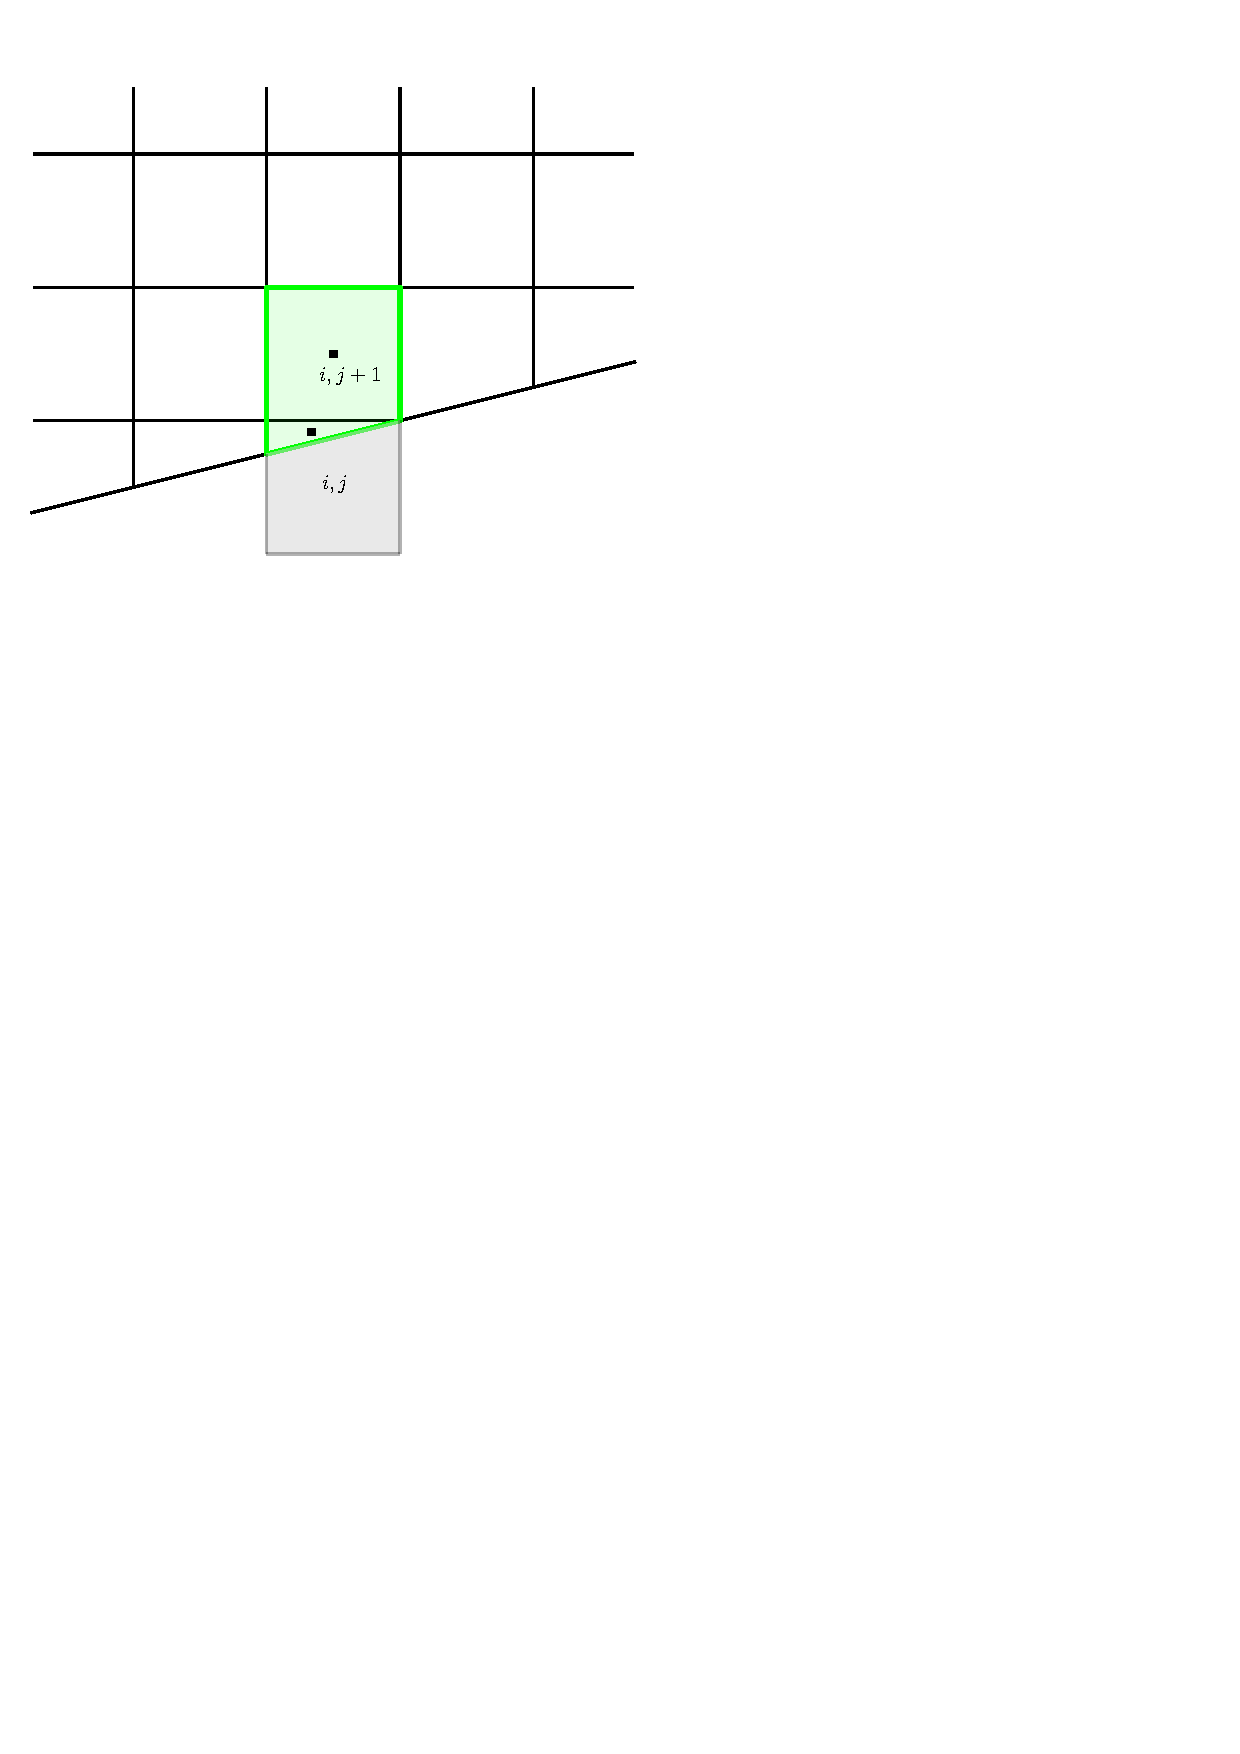
\includegraphics[width=.45\textwidth]{figs/modelexample2D_2.pdf} \label{fig:2nborTile2}}
	\caption{\sf Two-dimensional example of overlapping neighborhoods.  The unweighted centroids of cells $i,j$ and $i,j+1$ are indicated with solid squares ($\blacksquare$).} \label{fig:2nborTile}
\end{figure}


\subsection{Limiting on merging neighborhoods}
In this section we design a linearity preserving limiter for slopes on merging neighborhoods.  Designing a limiter that does not destroy the linearly preserving property is not so straightforward.  
%We demonstrate this
%In particular, we apply the LP limiter [] on slopes
